\documentclass[epsfig,10pt,fullpage]{article}

\newcommand{\LabNum}{3}
\newcommand{\CommonDocsPath}{../../common/docs}
\addtolength{\textwidth}{1.5in}
\addtolength{\oddsidemargin}{-0.75in}
\addtolength{\topmargin}{-0.75in}
\addtolength{\textheight}{1.5in}
\addtolength{\evensidemargin}{0.75in}
\setlength\parindent{0pt}
\raggedbottom

\usepackage{ae,aecompl}
\usepackage{epsfig,float,times}
\usepackage[hypcap]{caption}
\usepackage[pdftex, colorlinks]{hyperref}
\usepackage{graphicx}
\usepackage[usenames, dvipsnames]{color}
\usepackage{rotating}
\usepackage{tikz}
\usetikzlibrary{automata,positioning}
\usepackage{placeins}

\widowpenalty 10000
\clubpenalty 10000

\newcommand{\red}[1]{{\color{red}\sf{#1}}}
\newcommand{\green}[1]{{\color{green}\sf{#1}}}
\newcommand{\blue}[1]{{\color{blue}\sf{#1}}}
\definecolor{PineGreen}{rgb}{0.0, 0.47, 0.44}
\definecolor{ForestGreen}{rgb}{0.13, 0.55, 0.13}
\definecolor{Brown}{rgb}{0.59, 0.29, 0.0}

\newcommand{\UPDatePublished}{Oct 2021}
\newcommand{\versnum}{21.1} %version number quartus/AMP
\newcommand{\quartusname}{Quartus\textsuperscript{\textregistered} Prime}	
\newcommand{\UPTextBar}{For \quartusname{} \versnum{}}
\newcommand{\thisyear}{2021 } %for copyright
\newcommand{\company}{FPGAcademy.org}
\newcommand{\longteamname}{FPGAcademy.org}
\newcommand{\teamname}{FPGAcademy}
\newcommand{\website}{FPGAcademy.org}

\newcommand{\productAcronym}{AMP}
\newcommand{\productNameShort}{Monitor Program}

\newcommand{\productNameMedTM}{A Monitor Program}
\newcommand{\productNameMed}{A Monitor Program}

%\newcommand{\headerLogoFilePath}[1]{#1/FPGAcademy.png}

% listings is a package that supports encapsulating source code in LaTeX conveniently
\usepackage{listings}

\def\expandparam\lstinputlisting[#1]#2{\edef\tmp{\noexpand\lstinputlisting[#1]{#2}}\tmp}

%%%%%%%%%%%%%%%%%%%% Source Code Formatting %%%%%%%%%%%%%%%%%%%%
\definecolor{globalCommentColour}{rgb}{0.588,0.588,0.588}

%%%%%%%%%%%%%%%%%%%%%%%%%%%%%%%%%%%%%%%%%%%%%%%%%%%%
% Defining language style
% NiosII ASM
\lstdefinelanguage[NiosII]{Assembler} {
  morekeywords={add, addi, and, andhi, andi, beq, bge, bgeu, bgt, bgtu, ble,  bleu, blt, bltu, bne, br, break,
  bret, call, callr, cmpeq, cmpeqi, cmpge, cmpgei, cmpgeu, cmpgeui, cmpgt, cmpgti, cmpgtu, cmpgtui, cmple,
  cmplei, cmpleu, cmpleui, cmplt, cmplti, cmpltu, cmpltui, cmpne, cmpnei, custom, div, divu, eret, flushd,
  flushda, flushi, flushp, initd, initda, initi, jmp, jmpi, ldb, ldbio, ldbu, ldbuio, ldh, ldhio, ldhu, ldhuio,
  ldw, ldwio, mov, movhi, movi, movia, movui, mul, muli, mulxss, mulxsu, mulxuu, nextpc, nop, nor, or, orhi, ori,
  rdctl, rdprs, ret, rol, roli, ror, sll, slli, sra, srai, srl, srli, stb, stbio, sth, sthio, stw, stwio,
  sub, subi, sync, trap, wrctl, wrtcl, wrprs, xor, xori, xorhi, xori},
  morekeywords=[2]{.abort, .ABORT, .align, .app-file, .ascii, .asciz, .balign, .byte, .comm, .data, .def,
  .desc, .dim, .double, .eject, .else, .end, .endef, .endif, .equ, .equiv, .err, .extern, .file, .fill, .float,
  .global, .globl, .hword, .ident, .if, .include, .int, .irp, .irpc, .lcomm, .lflags, .line, .linkonce, .ln,
  .list, .long, .macro, .mri, .nolist, .octa, .org, .p2align, .psize, .quad, .rept, .sbttl, .scl, .section,
  .set, .short, .single, .size, .sleb128, .skip, .space, .stadb, .stabn, .stabs, .string, .symver, .tag,
  .text, .title, .type, .val, .uleb128, .word},
  morekeywords=[3]{et, bt, gp, sp, fp, ea, sstatus, ra, pc, status, estatus, bstatus, ienable, ipending, cpuid,
  exception, pteaddr, tlbacc, tlbmisc, eccinj, badaddr, config, mpubase, mpuacc},
  sensitive=t,
  alsoletter=.,
  morestring=[b]",
  morecomment=[s]{/*}{*/},
  morecomment=[l]\#,
}[keywords,comments,strings]
   
%% NOTE: morekeywords=[2] are GNU directives.
   
\definecolor{niosInstructionColour}{rgb}{0.000,0.608,0.000}
\definecolor{niosDirectiveColour}{rgb}{0.000,0.000,0.902}
\definecolor{niosSpecialRegColour}{rgb}{0.000,0.000,0.000}
\definecolor{niosStringColour}{rgb}{0.808,0.482,0.000}
   
%% NOTE: To make bold use: =\bfseries\color{<colour>}
\lstdefinestyle{defaultNiosStyle} {
  language=[NiosII]{Assembler},
  stringstyle=\color{niosStringColour},
  keywordstyle=\color{niosInstructionColour},
  keywordstyle=[2]\color{niosDirectiveColour},
  keywordstyle=[3]\itshape\color{niosSpecialRegColour}
}
%%%%%%%%%%%%%%%%%%%%%%%%%%%%%%%%%%%%%%%%%%%%%%%%%%%%

%%%%%%%%%%%%%%%%%%%%%%%%%%%%%%%%%%%%%%%%%%%%%%%%%%%%
% Defining language style
% ArmA9 ASM
\lstdefinelanguage[ArmA9]{Assembler} {
  morekeywords={ADC, ADD, ADDS, AND, ANDS, B, BAL, BEQ, BGE, BGT, BL, BLT, BIC, BKPT, BLX, BNE, BX, CDP, CLZ, CMN, CMP, EOR,
  EORS, LDC, LDM, LDR, LDRB, LDRBT, LDRH, LDRSB, LDRSH, LDRT, LSL, MCR, MLA, MOV, MOVW, MOVT, MRC, MRS, MSR, MUL, MVN, ORR, PLD,
  ROR, RSB, RSC, SBC, SMLAL, SMULL, STC, STM, STR, STRB, STRBT, STRH, STRT, SUB, SUBS, SWI, SWP, SWPB, TEQ, UMLAL,
  PUSH, POP, MOVS, RORS, LSR},
  morekeywords=[2]{.abort, .ABORT, .align, .app-file, .ascii, .asciz, .balign, .byte, .comm, .data, .def,
  .desc, .dim, .double, .eject, .else, .end, .endef, .endif, .equ, .equiv, .err, .extern, .file, .fill, .float,
  .global, .globl, .hword, .ident, .if, .include, .int, .irp, .irpc, .lcomm, .lflags, .line, .linkonce, .ln,
  .list, .long, .macro, .mri, .nolist, .octa, .org, .p2align, .psize, .quad, .rept, .sbttl, .scl, .section,
  .set, .short, .single, .size, .sleb128, .skip, .space, .stadb, .stabn, .stabs, .string, .symver, .tag,
  .text, .title, .type, .val, .vectors, .uleb128, .word},
  morekeywords=[3]{SP, PC, MIDR, CTR, TCMTR, TLBTR, MPIDR, ID_PFR0, ID_PFR1, ID_DFR0, ID_MMFR0, ID_MMFR1, ID_MMFR2,
  ID_MMFR3, ID_ISAR0, ID_ISAR1, ID_ISAR2, ID_ISAR3, ID_ISAR4, CCSIDR, CLIDR, AIDR, CSSELR, TTBR0, TTRB1, TTBR2, DACR,
  DFSR, IFSR, ADFSR, AIFSR, DFAAR, IFAR, ICIALLUIS, BPIALLIS, PAR, ICIALLU, ICIMVAU, BPIALL, DCIMVAC, DCISW, V2PCWPR,
  DCCVAC, DCCSW, DDIMVAC, DCISW, TLBALLIS, TLBIMVAIS, TLBIASIDIS, TLBIMVAAIS, TLBIALL, TLBIMVA, TLBIASID, TLBIMVAA,
  PMCR, PMCNTENSET, PMCNTENCLR, PMOVSR, PMSWINC, PMSELR, PMXEVTYPER, PMXEVCNTR, PMUSERENR, PMINTENSET, PMINTENCLR,
  PRRR, NRRR, PLEIDR, PLEASR, PLEFSR, PLEUAR, PLEPCR, VBAR, MVBAR, ISR, FCSEIDR, CONTEXTIDR, TPIDRURW, TPIDRURO, TPIDRPRW},
  sensitive=f,
  alsoletter=.,
  morestring=[b]",
  morecomment=[s]{/*}{*/},
  morecomment=[l]{//},
}[keywords,comments,strings]
   
%% NOTE: morekeywords=[2] are GNU directives.
   
\definecolor{armInstructionColour}{rgb}{0.000,0.608,0.000}
\definecolor{armDirectiveColour}{rgb}{0.000,0.000,0.902}
\definecolor{armSpecialRegColour}{rgb}{0.000,0.000,0.000}
\definecolor{armStringColour}{rgb}{0.808,0.482,0.000}
   
\lstdefinestyle{defaultArmStyle} {
  language=[ArmA9]{Assembler},
  stringstyle=\color{armStringColour},
  keywordstyle=\color{armInstructionColour},
  keywordstyle=[2]\color{armDirectiveColour},
  keywordstyle=[3]\itshape\color{armSpecialRegColour}
}
%%%%%%%%%%%%%%%%%%%%%%%%%%%%%%%%%%%%%%%%%%%%%%%%%%%%

%%%%%%%%%%%%%%%%%%%%%%%%%%%%%%%%%%%%%%%%%%%%%%%%%%%%
% Defining language style
% FPGAcademy ASM
\lstdefinelanguage{ASM}{
  morekeywords = [1]{mv, mvt, mvne, mvcc, add, sub, st, ld, and, b, bne, beq, bcc, bcs},
  morekeywords = [2]{word, define},
  keywordstyle = [1]\color{ForestGreen},
  keywordstyle = [2]\color{blue},
  sensitive = true,
  morecomment = [l]{//},
}

\lstset{
  language = ASM,
  basicstyle=\small\color{black}\ttfamily,
  commentstyle=\small\color{Brown}\itshape\ttfamily,
  showstringspaces=false,
  frame=none, %lines % boxed listings
  breaklines=true,
  breakatwhitespace=true,
  tabsize=3
}
%%%%%%%%%%%%%%%%%%%%%%%%%%%%%%%%%%%%%%%%%%%%%%%%%%%%

%%%%%%%%%%%%%%%%%%%%%%%%%%%%%%%%%%%%%%%%%%%%%%%%%%%%
% Defining language style
% Java
\definecolor{javaStringColour}{rgb}{0.808,0.482,0}
%%%%%%%%%%%%%%%%%%%%%%%%%%%%%%%%%%%%%%%%%%%%%%%%%%%%

%%%%%%%%%%%%%%%%%%%%%%%%%%%%%%%%%%%%%%%%%%%%%%%%%%%%
% Defining language style
% C
\definecolor{CStringColour}{rgb}{0.808,0.482,0}

\lstset{
  language = C,
  basicstyle=\small\color{black}\ttfamily, 
  commentstyle=\small\color{PineGreen}\itshape\ttfamily,
  keywordstyle=\small\color{blue}\bfseries\ttfamily,
  showstringspaces=false,
  frame=none, %lines % boxed listings
  breaklines=true,
  breakatwhitespace=true,
  tabsize=3
}
%%%%%%%%%%%%%%%%%%%%%%%%%%%%%%%%%%%%%%%%%%%%%%%%%%%%

%%%%%%%%%%%%%%%%%%%%%%%%%%%%%%%%%%%%%%%%%%%%%%%%%%%%
% Defining language style
% Verilog
\definecolor{verilogCommentColour}{rgb}{0.000,0.502,0.000}

\lstdefinestyle{defaultVerilogStyle} {
  language={Verilog},
  keywordstyle=\color{blue},
  commentstyle=\color{verilogCommentColour}
}
%%%%%%%%%%%%%%%%%%%%%%%%%%%%%%%%%%%%%%%%%%%%%%%%%%%%

%%%%%%%%%%%%%%%%%%%%%%%%%%%%%%%%%%%%%%%%%%%%%%%%%%%%
% Defining language style
% VHDL
\lstdefinestyle{defaultVHDLStyle} {
  language={VHDL},
  keywordstyle=\color{blue},
  commentstyle=\color{verilogCommentColour}
}
%%%%%%%%%%%%%%%%%%%%%%%%%%%%%%%%%%%%%%%%%%%%%%%%%%%%

%%%%%%%%%%%%%%%%%%%%%%%%%%%%%%%%%%%%%%%%%%%%%%%%%%%%
% Defining language style
% LaTeX
\lstdefinelanguage[LocalLaTeX]{TeX}[LaTeX]{TeX}{moretexcs={bf, it, sf, lstset},}

\lstdefinestyle{defaultLocalLatexStyle} {
  language=[LocalLatex]{TeX},
  keywordstyle=\color{blue}\bfseries,
  keywordstyle=[2]\color{blue},
  keywordstyle=[3]\color{blue}\bfseries
}
%%%%%%%%%%%%%%%%%%%%%%%%%%%%%%%%%%%%%%%%%%%%%%%%%%%%

%%%%%%%%%%%%%%%%%%%%%%%%%%%%%%%%%%%%%%%%%%%%%%%%%%%%
% Defining language style
% Default
\lstset{
  basicstyle=\small\color{black}\ttfamily,
  commentstyle=\small\color{globalCommentColour}\itshape\ttfamily,
  keywordstyle=\small\color{blue}\bfseries\ttfamily,
  showstringspaces=false,
  frame=none, %lines % boxed listings
  breaklines=true,
  breakatwhitespace=true,
  tabsize=3
}
%%%%%%%%%%%%%%%%%%%%%%%%%%%%%%%%%%%%%%%%%%%%%%%%%%%%


\hypersetup{
  pdftitle={Embedded Systems Lab Exercise \LabNum},
  linkcolor=blue,
  hyperindex=true,
  pdfauthor={FPGAcademy.org},
  pdfkeywords={FPGAcademy.org, FPGAcademy, Lab, Exercise, Embedded Systems},
  bookmarks,
  bookmarksopen=false,
  filecolor=blue,
  pdfstartview={FitH},
  urlcolor=blue,
  plainpages=false,
  pdfpagelabels=true,
  linkbordercolor={1 1 1} %no color for link border
}



\begin{document}

\centerline{\huge Embedded Systems}
~\\
\centerline{\huge Laboratory Exercise \LabNum}
~\\
\centerline{\large Character Device Drivers}

\section*{Part I}
\noindent
The purpose of this laboratory exercise is to teach you how to write and implement character 
device drivers. {\it Character device drivers} are kernel modules that provide a file-based 
interface to user-level programs. When a character device driver is inserted into the 
Linux* kernel, a special type of file associated with the driver is created, usually in the 
filesystem folder /{\it dev}. For example, if the driver is named {\it chardev} then the 
associated file would be /{\it dev}/{\it chardev}. A user-level program can read or write to 
this file to communicate with the driver. In this exercise we will develop a character
device driver that can communicate with the user to print different text strings on the
Terminal window. While this is not an especially interesting driver, it will serve to illustrate 
how the code for a character device driver has to be structured. In later laboratory exercises we
will use the knowledge developed here to write drivers that perform more useful functions,
such as controlling hardware devices like switches, pushbuttons, LEDs, timers, video and
audio output, and an accelerometer.

~\\
\noindent
An example of code for a character device driver is given in Figure~\ref{fig:chardev}.
This is a trivial example that is meant to illustrate how the code for a driver has to be
structured. If a user reads from this driver, it simply replies with the text
\texttt{Hello from chardev}. One way to read from the driver is to execute the Linux command
\texttt{cat /dev/chardev}. This driver supports both reading and writing.
The user can change the character string provided by the driver
by writing to it. One way to write to the driver is to use the Linux command
\texttt{echo "New message" > /dev/chardev}.

~\\
\noindent
Linux provides a number of programming interfaces that can be used to specify a character device
driver. For this exercise we will use an interface that is intended for making 
{\it miscellaneous} drivers for custom hardware. The driver can be specified by using some 
special types of variables and data structures, as well as a library function that 
{\it registers} the driver in the Linux kernel.  Important lines of code in
Figure~\ref{fig:chardev} are described below. Lines~\ref{line:inc1} to \ref{line:inc2} 
include some header files that are required for character device drivers.
Lines~\ref{line:dec1} to \ref{line:dec2} provide prototype declarations for the 
functions \texttt{device\_open}, \texttt{device\_release},
\texttt{device\_read}, and \texttt{device\_write}. These are the functions that will be 
called by the Linux kernel when a user program performs an open, close, read, or write 
operation, respectively, on the file /{\it dev}/{\it chardev}. To support these functions
the driver declares the variable {\it chardev}\_{\it fops} in Line~\ref{line:fops}, which 
has the type \texttt{struct file\_operations}. It provides references to the functions from 
Lines~\ref{line:dec1} to \ref{line:dec2}.

~\\
\noindent
Line~\ref{line:miscdev} declares a variable named {\it chardev}, which is used to
represent our character device driver. It has the type \texttt{struct miscdevice}. 
For our character device driver the fields .{\it minor} and .{\it mode} can be set 
to the values shown in this example. The .{\it name} field specifies the name of the driver,
which is {\it chardev} in this example. Finally, the .{\it fops} field contains a pointer
to the driver's \texttt{file\_operations} data structure.

~\\
\noindent
The driver is created in the {\it start}\_{\it chardev} function shown
in lines~\ref{line:s0} to~\ref{line:s1}. It calls the Linux library function 
{\it misc}\_{\it register} with an argument that is a pointer to the {\it chardev} variable. 
If this function returns a value $\geq 0$, then the character device driver will have been 
successfully created by the Linux kernel.
The \texttt{start\_chardev} function is executed when the character
device driver is {\it inserted} into the Linux kernel. When this driver is removed from the
kernel, the function \texttt{stop\_chardev} is called, shown in lines~\ref{line:code5}
to~\ref{line:code6}. Note that it is possible to print error or debug information on the 
Linux terminal window, by calling the {\it printk} kernel function. This function
works similarly to the C library function {\it printf}, and has the same types of formatting 
options. Examples of {\it printk} are shown in Lines~\ref{line:s2} and~\ref{line:s3}.
When {\it printk} is given the \texttt{KERN\_ERR} argument, its output appears on the
Linux Terminal window. But if the \texttt{KERN\_INFO} argument is used, then the output is
stored into a Linux {\it log} file. You can examine the content of this log file by executing the
Linux command \texttt{dmesg}.

\lstset{language=C,numbers=left,escapechar=|}
\begin{figure}[H]
\begin{center}
\begin{minipage}[t]{15 cm}
\begin{lstlisting}[name=chardev]
|\label{line:inc1}|#include <linux/fs.h>           // struct file, struct file_operations
#include <linux/module.h>       // for module init and exit macros
#include <linux/miscdevice.h>   // for misc_device_register and struct miscdev
|\label{line:inc2}|#include <asm/io.h>  

/* Kernel character device driver /dev/chardev. */
|\label{line:dec1}|static int device_open (struct inode *, struct file *);
static int device_release (struct inode *, struct file *);
static ssize_t device_read (struct file *, char *, size_t, loff_t *);
|\label{line:dec2}|static ssize_t device_write(struct file *, const char *, size_t, loff_t *);

|\label{line:fops}|static struct file_operations chardev_fops = {
    .owner = THIS_MODULE,
    .read = device_read,
    .write = device_write,
    .open = device_open,
    .release = device_release
};

#define SUCCESS 0
#define DEV_NAME "chardev"

|\label{line:miscdev}|static struct miscdevice chardev = { 
    .minor = MISC_DYNAMIC_MINOR, 
    .name = DEV_NAME,
    .fops = &chardev_fops,
    .mode = 0666
};
|\label{line:check}|static int chardev_registered = 0;

#define MAX_SIZE 256	// assume that no message longer than this will be used
|\label{line:code20}|static char chardev_msg[MAX_SIZE];	// the string that can be read or written

|\label{line:s0}|static int __init start_chardev(void) {
    |\label{line:devnum}|int err = misc_register (&chardev);
    if (err < 0) {
        |\label{line:s2}|printk (KERN_ERR "/dev/%s: misc_register() failed\n", DEV_NAME);
    }
    else {
        |\label{line:s3}|printk (KERN_INFO "/dev/%s driver registered\n", DEV_NAME);
        chardev_registered = 1;
    }
    |\label{line:code4a}|strcpy (chardev_msg, "Hello from chardev\n"); 

    return err;
|\label{line:s1}|}

|\label{line:code5}|static void __exit stop_chardev(void) {
    if (chardev_registered) {
        misc_deregister (&chardev);
        printk (KERN_INFO "/dev/%s driver de-registered\n", DEV_NAME);
    }
|\label{line:code6}|}
\end{lstlisting}
\end{minipage}
\caption{The character device driver code. (Part $a$)}
\label{fig:chardev}
\end{center}
\end{figure}

\lstset{language=C,numbers=left,escapechar=|,firstnumber=auto,name=chardev}
\begin{center}
\begin{minipage}[t]{15 cm}
\begin{lstlisting}[name=chardev]
|\label{line:code7}|/* Called when a process opens chardev */
static int device_open(struct inode *inode, struct file *file) {
    return SUCCESS;
}

/* Called when a process closes chardev */
static int device_release(struct inode *inode, struct file *file) {
    return 0;
|\label{line:code8}|}

|\label{line:code9}|/* Called when a process reads from chardev. Provides character data from 
 * chardev_msg. Returns, and sets *offset to, the number of bytes read. */
static ssize_t device_read(struct file *filp, char *buffer, size_t length, loff_t *offset) {
    size_t bytes;
    |\label{line:code11}|bytes = strlen (chardev_msg) - (*offset);  // how many bytes not yet sent?
    |\label{line:code12}|bytes = bytes > length ? length : bytes;   // too much to send at once?
    
    if (bytes)
        |\label{line:code13}|(void) copy_to_user (buffer, &chardev_msg[*offset], bytes);
    |\label{line:code14}|*offset = bytes;	// keep track of number of bytes sent to the user
    |\label{line:code15}|return bytes;
|\label{line:code10}|}

|\label{line:code16}|/* Called when a process writes to chardev. Stores the data received into
 * chardev_msg, and returns the number of bytes stored. */
static ssize_t device_write(struct file *filp, const char *buffer, size_t length, loff_t *offset) {
    size_t bytes;
    bytes = length;

    |\label{line:code18}|if (bytes > MAX_SIZE - 1)	// can copy all at once, or not?
        bytes = MAX_SIZE - 1;
    |\label{line:code19}|(void) copy_from_user (chardev_msg, buffer, bytes);
    chardev_msg[bytes] = '\0';	// NULL terminate
    // Note: we do NOT update *offset; we keep the last MAX_SIZE or fewer bytes
    return bytes;
|\label{line:code17}|}

MODULE_LICENSE("GPL");
module_init (start_chardev);
module_exit (stop_chardev);
\end{lstlisting}
\end{minipage}
\end{center}
\begin{center}
~\\
Figure \ref{fig:chardev}. The character device driver code. (Part $b$)
\end{center}

\noindent
Lines~\ref{line:code7} to~\ref{line:code8} in Figure~\ref{fig:chardev}
give the code for \texttt{device\_open} and
\texttt{device\_release}. For most character device drivers nothing needs to be done in these
functions, and hence the code simply {\it returns}.
Lines~\ref{line:code9} to~\ref{line:code10} show the \texttt{device\_read} function. The
first argument to this function, \texttt{filp}, is not used in this example. The second argument,
\texttt{buffer}, is used to pass character data from the driver back to the 
user-level process that read from /{\it dev}/{\it chardev}.
The \texttt{length} argument specifies the maximum number of bytes that can be stored 
in the \texttt{buffer}. The final argument, \texttt{offset}, will be discussed later. 
Lines~\ref{line:code11} to~\ref{line:code12} determine how much data can be sent back to
the kernel. If \texttt{length} is greater than \texttt{bytes} then the whole message can
be sent at once. Otherwise only \texttt{length} characters can be sent. The value of
\texttt{bytes} is calculated in Line~\ref{line:code11}. 

~\\
\noindent
To understand the way that the \texttt{offset} variable determines how many bytes are
returned to the user in the read operation, consider the following scenario. 
When a user opens the file /{\it dev}/{\it chardev}, and then performs a read from the 
file, \texttt{*offset} will be 0. Thus, \texttt{bytes} for this read operation will be set 
to the length of the character string that is returned when the driver is read.
In Linux the kernel does not directly access the memory addresses, or variables, in
a user-level program. Similarly, user-level code cannot access memory addresses within
the kernel. The kernel provides special functions for passing data between 
itself and user-level programs. One such function, \texttt{copy\_to\_user},
is called in Line~\ref{line:code13} of Figure~\ref{fig:chardev}. It copies character data
from the kernel back to the user-level program via the \texttt{buffer}. The kernel variable
\texttt{offset} is set to the value of the variable \texttt{bytes} in 
line~\ref{line:code14}. This value of \texttt{offset},
associated with /{\it dev}/{\it chardev}, is stored in the kernel as long as the file
remains open. In line~\ref{line:code15} the \texttt{device\_read} function provides 
as a return value the number of bytes stored into the \texttt{buffer}. A typical
user-level program that reads from the device driver (e.g., \texttt{cat /dev/chardev})
will read from the file until \texttt{device\_read} returns 0, which indicates {\it
end-of-file}. The way this works in our example is as follows. The first time
\texttt{device\_read} is called it copies the character string back to the
\texttt{buffer} and returns the {\it string length}. But a second call to 
\texttt{device\_read} will copy nothing into the \texttt{buffer} and will return 0. This
mechanism is facilitated by the way in which \texttt{offset} is used in the code.

~\\
\noindent
Lines~\ref{line:code16} to~\ref{line:code17} show the \texttt{device\_write} function. The
first argument to this function, \texttt{filp}, is not used in this example. The second argument,
\texttt{buffer}, is used to get character data from the user program into the device driver.
The \texttt{length} argument specifies the amount of data that is to be transferred.
The \texttt{offset} argument is not used in this example.
Data transferred from the user is stored into \texttt{chardev\_msg}, overwriting the
previous message.
Line~\ref{line:code18} checks for overflow, so that the amount of data can be reduced if needed. 
In line~\ref{line:code19} the kernel function \texttt{copy\_from\_user} is called to get
the user-data and copy it into \texttt{chardev\_msg}. 

~\\
The \texttt{device\_write} function provides as a return value the number of bytes copied
into \texttt{chardev\_msg}. A typical user-level program (e.g., \texttt{echo "New message" 
> /dev/chardev}) will continue to call the \texttt{device\_write} function until a total 
of \texttt{length} bytes have been received by the driver. In our example each call to 
\texttt{device\_write} overwrites the data stored in \texttt{chardev\_msg}.

~\\
\noindent
Perform the following:

\begin{enumerate}
\item Create a C source-code file named {\it chardev.c} for the device driver code in 
Figure~\ref{fig:chardev}. The source code can be obtained from the design files that
accompany this lab exercise on the {\it FPGAcademy.org} website. 
\item Create a Makefile for your character device driver, following the format given in
the tutorial {\it Using Linux on DE-series Boards}. Compile the code to create the kernel module 
{\it chardev.ko}, and insert this module into the Linux kernel. 
Check the filesystem folder /{\it dev} to see that the file /{\it dev}/{\it chardev} was
created as a result of inserting your kernel module. Type the command \texttt{cat
/dev/chardev} and observe that your character device driver responds with the message
\texttt{Hello from chardev}. Overwrite the default message by typing a command such as
\texttt{echo "New Message" > /dev/chardev}. Then, issue the \texttt{cat} command again to
see that the driver responds with the new message.
\item
In addition to using commands like \texttt{cat} and \texttt{echo}, you can write your own
user-level programs that read and write to your character device driver. An example program 
is given in Figure~\ref{fig:part1}. It uses the kernel functions \texttt{open}, \texttt{read},
\texttt{write}, and \texttt{close} to communicate with the character device driver through
the file /{\it dev}/{\it chardev}. Create a C source-code file called {\it part1.c} for
this program, and compile it using a command such as \texttt{gcc -Wall -o part1 part1.c}.
The source code in Figure~\ref{fig:part1} is provided in the design files for this exercise.
Run the resulting executable program and observe the output that it produces.
\end{enumerate}

\lstset{language=C,numbers=none}
\begin{figure}[H]
\begin{center}
\begin{minipage}[t]{15 cm}
\begin{lstlisting}[name=part1]
#include <stdio.h>
#include <signal.h>
#include <string.h>
#include <errno.h>
#include <fcntl.h>
#include <unistd.h>

#define BYTES 256    // max # of bytes to read from /dev/chardev

volatile sig_atomic_t stop;
void catchSIGINT(int signum){
    stop = 1;
}

/* This code uses the character device driver /dev/chardev. The code reads the 
 * default message from the driver and then prints it. After this the code 
 * changes the message in a loop by writing to the driver, and prints each new
 * message. The program exits if it receives a kill signal (for example, ^C 
 * typed on stdin). */
int main(int argc, char *argv[])
{
    int chardev_FD;              // file descriptor
    char chardev_buffer[BYTES];  // buffer for chardev character data
    int ret_val, chars_read;     // number of characters read
    char new_msg[128];           // space for the new message
    int i_msg;
    
    // catch SIGINT from ^C, instead of having it abruptly close this program
    signal(SIGINT, catchSIGINT);
    
    // Open the character device driver for read/write
    if ((chardev_FD = open("/dev/chardev", O_RDWR)) == -1) {
        printf("Error opening /dev/chardev: %s\n", strerror(errno));
        return -1;
    }

    i_msg = 0;
    while (!stop) {
        chars_read = 0;
        while ((ret_val = read (chardev_FD, chardev_buffer, BYTES)) != 0)
            chars_read += ret_val;          // read the driver until EOF
        chardev_buffer[chars_read] = '\0';  // NULL terminate
        printf ("%s", chardev_buffer);

        sprintf (new_msg, "New message %d\n", i_msg);
        i_msg++;
        write (chardev_FD, new_msg, strlen(new_msg));

        sleep (1);
    }

    close (chardev_FD);
    return 0;
}
\end{lstlisting}
\end{minipage}
\caption{A program that communicates with /{\it dev}/{\it chardev}.}
\label{fig:part1}
\end{center}
\end{figure}

~\\
\noindent
An alternative version of the \texttt{read\_device} function is given in 
Figure~\ref{fig:alternate}. Instead of calling the kernel function
\texttt{copy\_to\_user}, this code copies one byte at a time by calling the kernel function
\texttt{put\_user}. Similarly, an alternative version of the \texttt{device\_write}
function that transfers one byte at a time instead of calling \texttt{copy\_from\_user}
is shown in Figure~\ref{fig:alternate}.  These alternative versions of the code 
are meant to provide additional examples of how device driver code can be written. The two
versions of the code perform exactly the same functions.

\lstset{language=C}
\begin{figure}[H]
\begin{center}
\begin{minipage}[t]{15 cm}
\begin{lstlisting}[name=alternate]
/* Called when a process reads from chardev. */
static ssize_t device_read(struct file *filp, char *buffer, size_t length, loff_t *offset) {
    size_t bytes_read = 0;
    char *msg_Ptr = &(chardev_msg[*offset]);
    
    // Write to user buffer
    while (length && *msg_Ptr)  {
        put_user(*(msg_Ptr++), buffer++);
        length--;
        bytes_read++;
    }
    (*offset) = bytes_read;
    return bytes_read;
}

/* Called when a process writes to chardev */
static ssize_t device_write(struct file *filp, const char *buffer, size_t length, loff_t *offset) {
    int i;

    for (i = 0; i < length; ++i)
        chardev_msg[i] = buffer[i];  // assume that data won't overflow
    chardev_msg[i] = '\0';           // NULL terminate
    return length;
}
\end{lstlisting}
\end{minipage}
\caption{Alternative versions of \texttt{device\_read} and \texttt{device\_write}}
\label{fig:alternate}
\end{center}
\end{figure}

\vspace{-1cm}
\section*{Part II}
\noindent
The discussion below assumes that the reader is using the DE1-SoC board. If you are using
the DE10-Standard board, then the same discussion applies. But if you are using the
DE10-Nano board, then some minor differences should be considered, because this 
board has fewer pushbutton KEYs and SW switches. 

~\\
\noindent
In some Linux systems user-level programs are not permitted to access the physical memory 
addresses of I/O devices. In such systems I/O devices can only be accessed via device
drivers. In this part you are to implement two character device drivers. One driver provides the
state of the KEY pushbutton switches in the DE1-SoC Computer, via the file 
/{\it dev}/{\it KEY}. The other driver provides the state of the SW slider switches, via
the file /{\it dev}/{\it SW}.

~\\
\noindent
Perform the following:

\begin{enumerate}
\item Create a new kernel module in a file {\it KEY\_SW.c}. Write the code for {\it both}
character device drivers in this module. Declare separate variables of type
\texttt{file\_operations} and \texttt{miscdevice} for each driver. 
Initialize each of these variables by
following the steps shown in Figure~\ref{fig:chardev}. When setting up the 
\texttt{file\_operations} data structure (see line~\ref{line:fops} in Figure~\ref{fig:chardev}), 
each of your character device drivers needs to have a function for \texttt{opening}, 
\texttt{releasing}, and \texttt{reading} its /{\it dev/file}. These drivers do not 
require a function for \texttt{writing}, since a user would not need to write anything 
to /{\it dev}/{\it KEY} or /{\it dev}/{\it SW}.

\noindent
Your module needs to have an initialization function, like the one beginning on Line~\ref{line:s0}
of Figure~\ref{fig:chardev}. If this function were named \texttt{init\_drivers}, then it 
would be declared using the syntax

\begin{lstlisting}
static int _|$\,$|_init init_drivers(void)
\end{lstlisting}

\noindent Your code has to identify the module initialization function by using the statement
\begin{lstlisting}
module_init (init_drivers);
\end{lstlisting}

\noindent
In {\it KEY\_SW.c} declare global variables that will hold virtual addresses for the KEY
and SW ports in the DE1-SoC Computer. Initialize these variables in
\texttt{init\_drivers}, using the kernel function \texttt{ioremap\_nocache}, as
illustrated in the tutorial {\it Using Linux on DE-series Boards}. Note that you do not need to 
use interrupts for this part of the exercise. 

\noindent
Write code for the \texttt{open}, \texttt{release}, and \texttt{read} functions for your drivers.
For the KEY driver you should read the state of the KEYs from the port's {\it Edgecapture} register.
The programmer registers in the KEY port of the DE1-SoC Computer are illustrated in
Figure~\ref{fig:KEY}. Return the KEY values to the user as {\it character} data (ASCII) in 
the \texttt{read} function for the KEY driver. One way to convert binary data into character 
data is to make use of a library function such as \texttt{sprintf}. You could encode the
binary data using ASCII in various schemes. For example, you could use one hexadecimal digit
to encode the data, and then send the ASCII value of that digit. If the KEY data were equal 
to \texttt{0011}, then you would return the character \texttt{3}, and if the data 
were \texttt{1111} you would return \texttt{F}. Choose whatever method you prefer for 
representing this data. For the SW driver, read the slider switch settings from the 
port's {\it Data} register, illustrated in Figure~\ref{fig:SW}. Return these values to the 
user in the form of {\it character} data, via the driver's \texttt{read} function. You can
choose to encode the 10 data bits in different ways. For example, if you use hexadecimal
and the data were \texttt{1100001010}, then you would return the ASCII characters
\texttt{30A}.

\begin{figure}[H]
   \begin{center}
       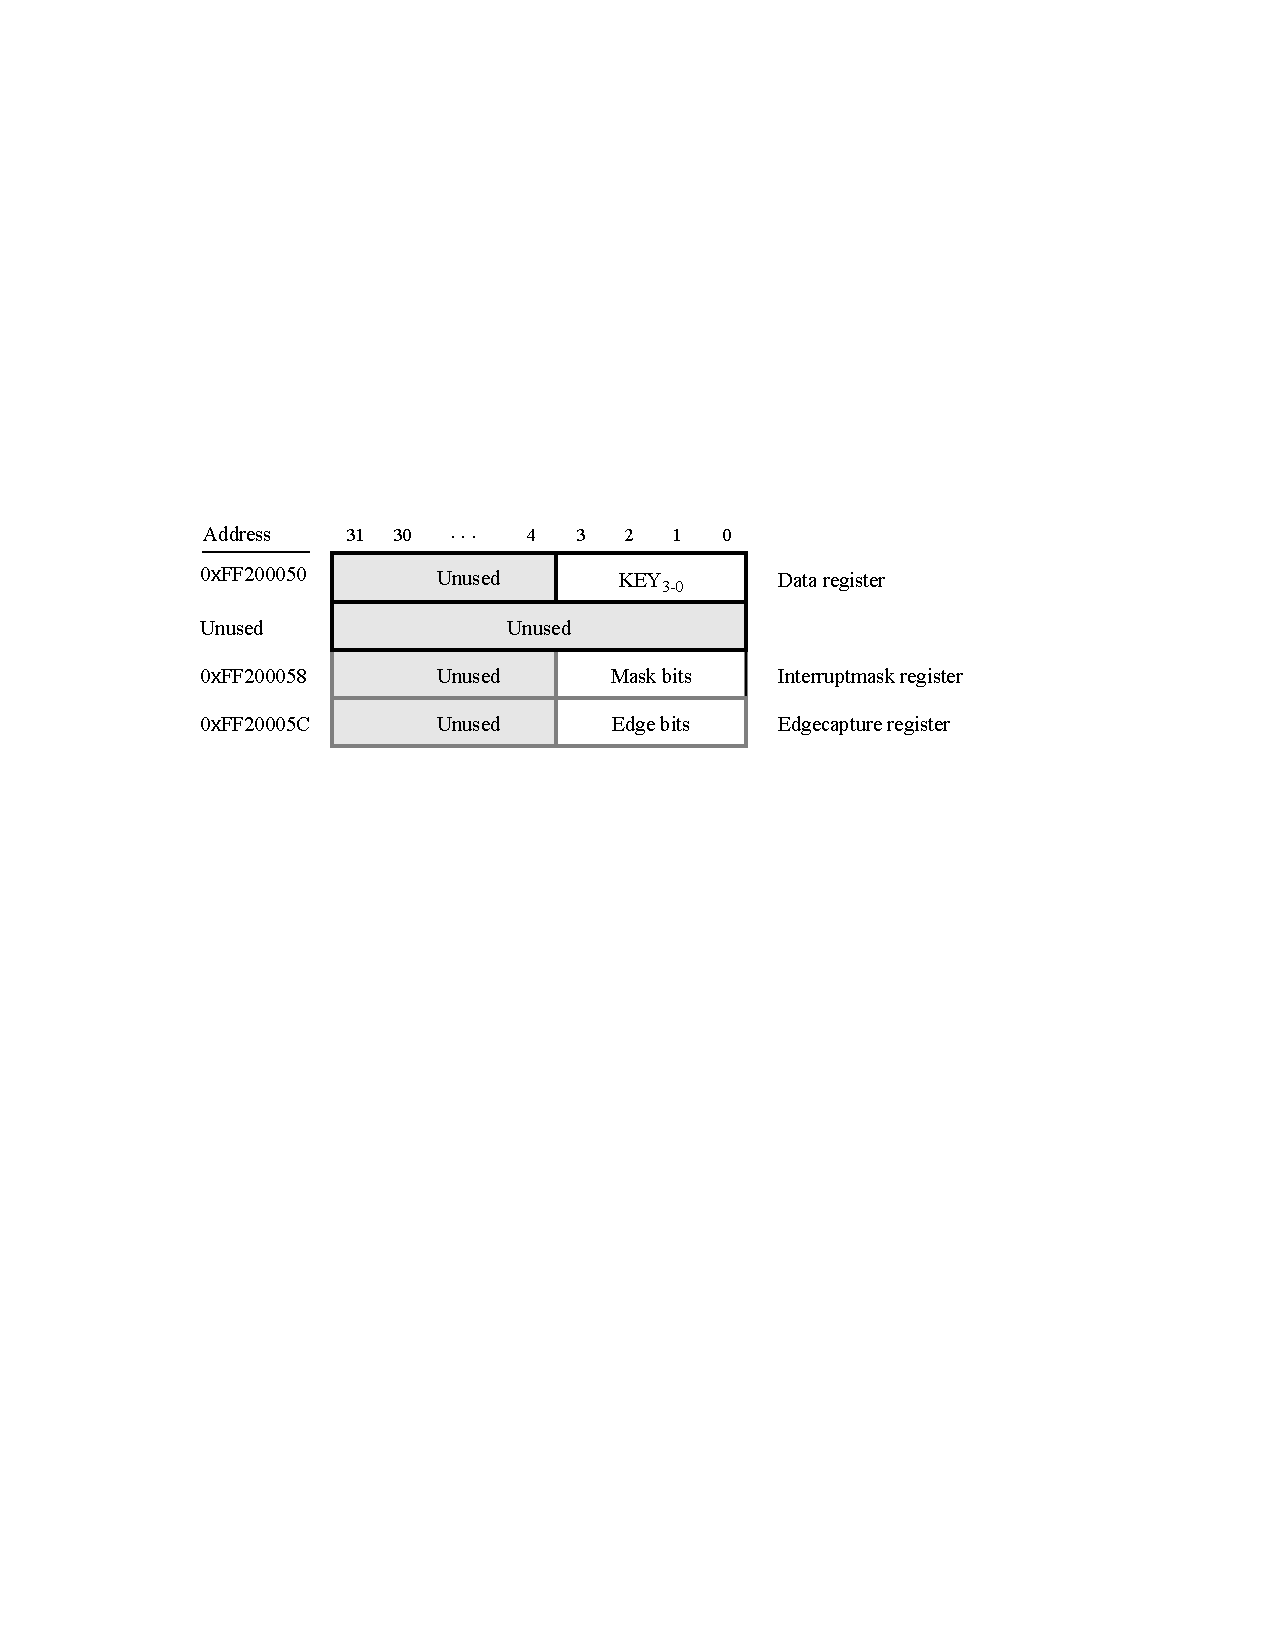
\includegraphics{figures/figureKEY.pdf}
   \end{center}
    \caption{The KEY pushbutton switch port.}
\label{fig:KEY}
\end{figure}

\begin{figure}[H]
   \begin{center}
       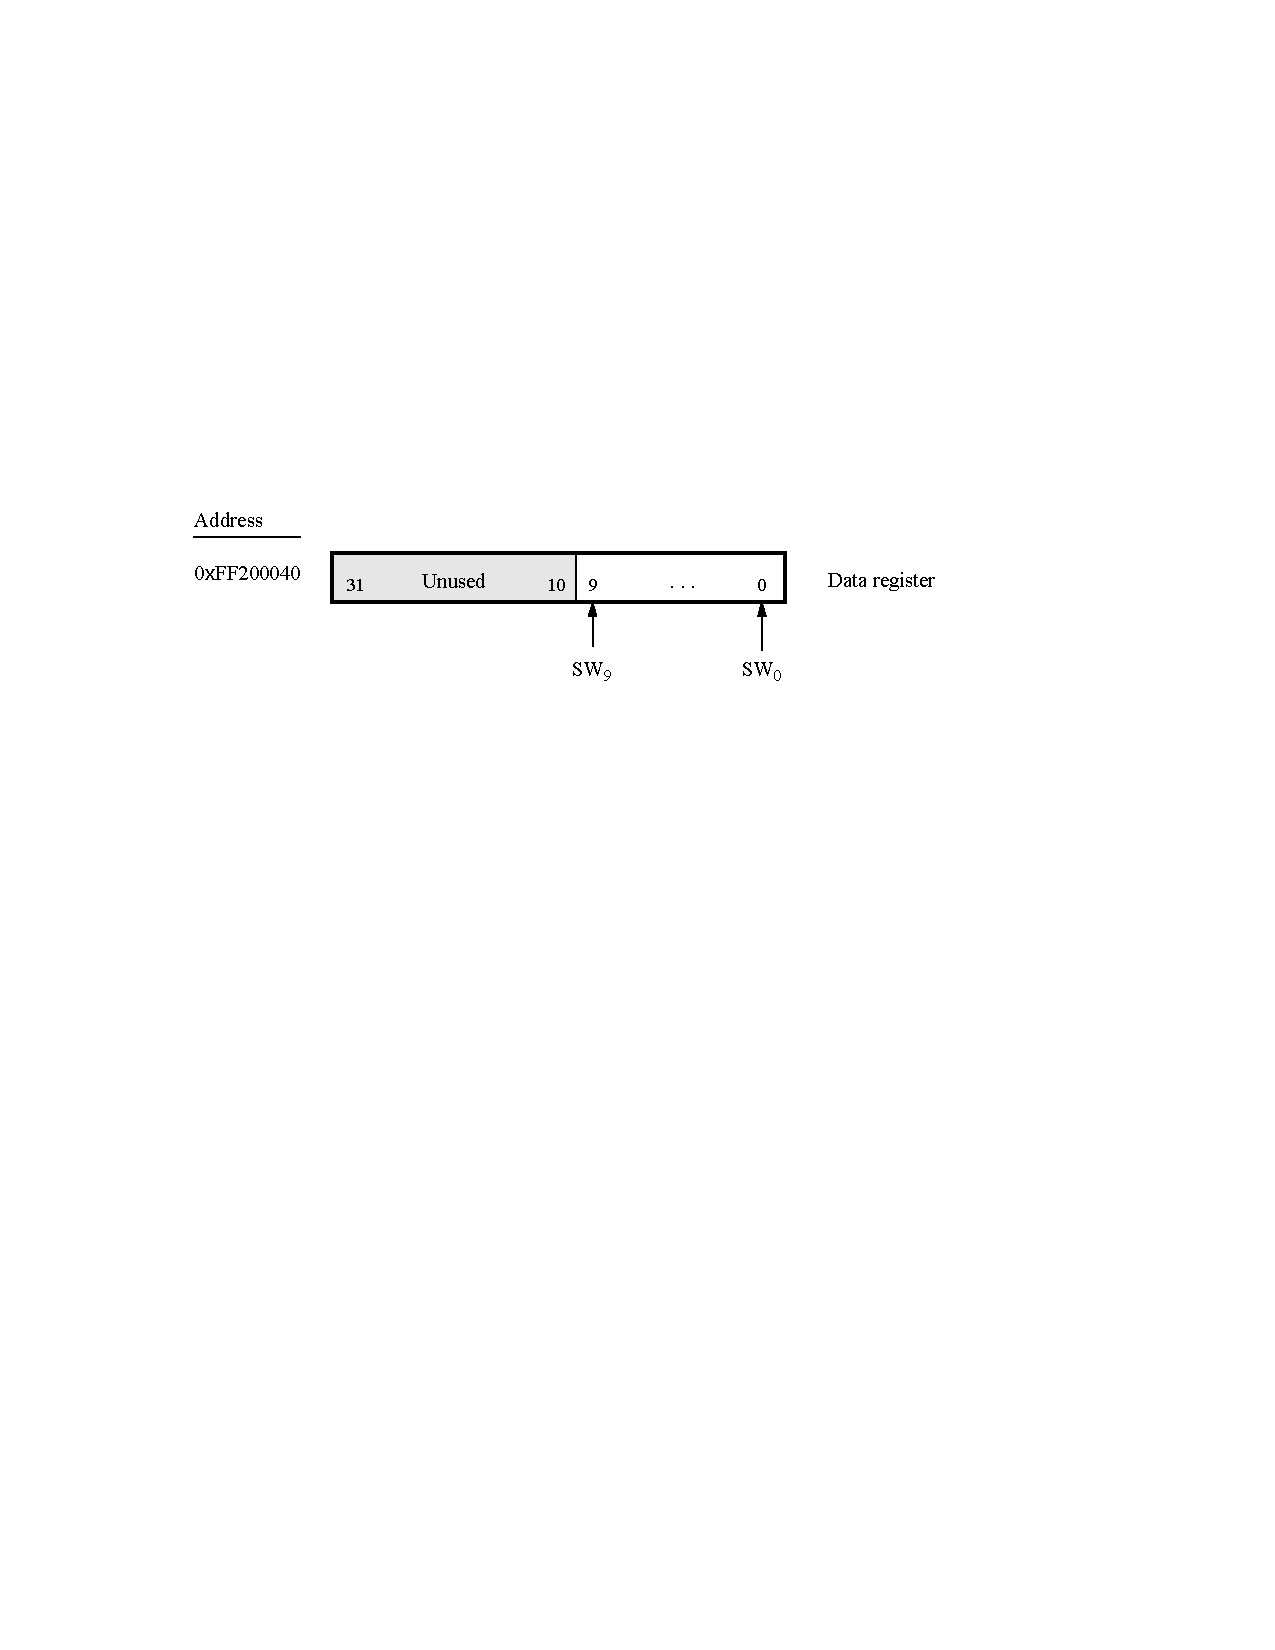
\includegraphics{figures/fig_slider_port.pdf}
   \end{center}
    \caption{The SW slider switch port.}
\label{fig:SW}
\end{figure}

\item Create a {\it Makefile} that can be used to compile your kernel module to produce the file 
{\it KEY\_SW.ko}. Insert this module into the kernel and verify that it creates the
character device files /{\it dev}/{\it KEY} and /{\it dev}/{\it SW}.

\item Test your drivers by using the commands \texttt{cat /dev/KEY} and \texttt{cat /dev/SW}.
Verify that the drivers provide correct values for the switches.
\end{enumerate}

\section*{Part III}
\noindent
This part of the exercise assumes that the reader is using the DE1-SoC board, to control
its LEDs and seven-segment displays. The same discussion applies for the DE10-Standard board.
But if the DE10-Nano board is being used instead, then two differences should be
considered: it has fewer LED lights, and it has no seven-segment displays. The reader can still 
perform the rest of the exercise, but should ignore any parts of the discussion that refer 
to seven-segment displays. 

~\\
\noindent
For this part you are to write another two character device drivers. One driver controls
the LEDR lights in the DE1-SoC Computer, via the file /{\it dev}/{\it LEDR}. The
other driver controls the seven-segment displays HEX5$-$HEX0, via the file /{\it dev}/{\it
HEX}. The LEDR port in the DE1-SoC Computer is illustrated in Figure~\ref{fig:LEDR}, and the
seven-segment display ports are depicted in Figure~\ref{fig:HEX}. Your driver should be 
able to display decimal digits $\red{0}-\red{9}$ on each of the six displays.
Perform the following:

\begin{enumerate}
\item Create a kernel module source-code file called {\it LEDR}\_{\it HEX.c}. Implement both
character device drivers in this module. For both drivers you should implement functions for
\texttt{open}, \texttt{release}, and \texttt{write} operations. These drivers do not require 
a \texttt{read} function.
\item Create a Makefile, compile your module, and insert it into the kernel.
\item Test the LEDR and HEX character device drivers by using the \texttt{echo} Linux command.
For example, if you designed your LEDR module to accept a three-digit hexadecimal value,
then the command \texttt{echo 3FF > /dev/LEDR} would turn on all ten LEDs.
\end{enumerate}

\begin{figure}[H]
   \begin{center}
       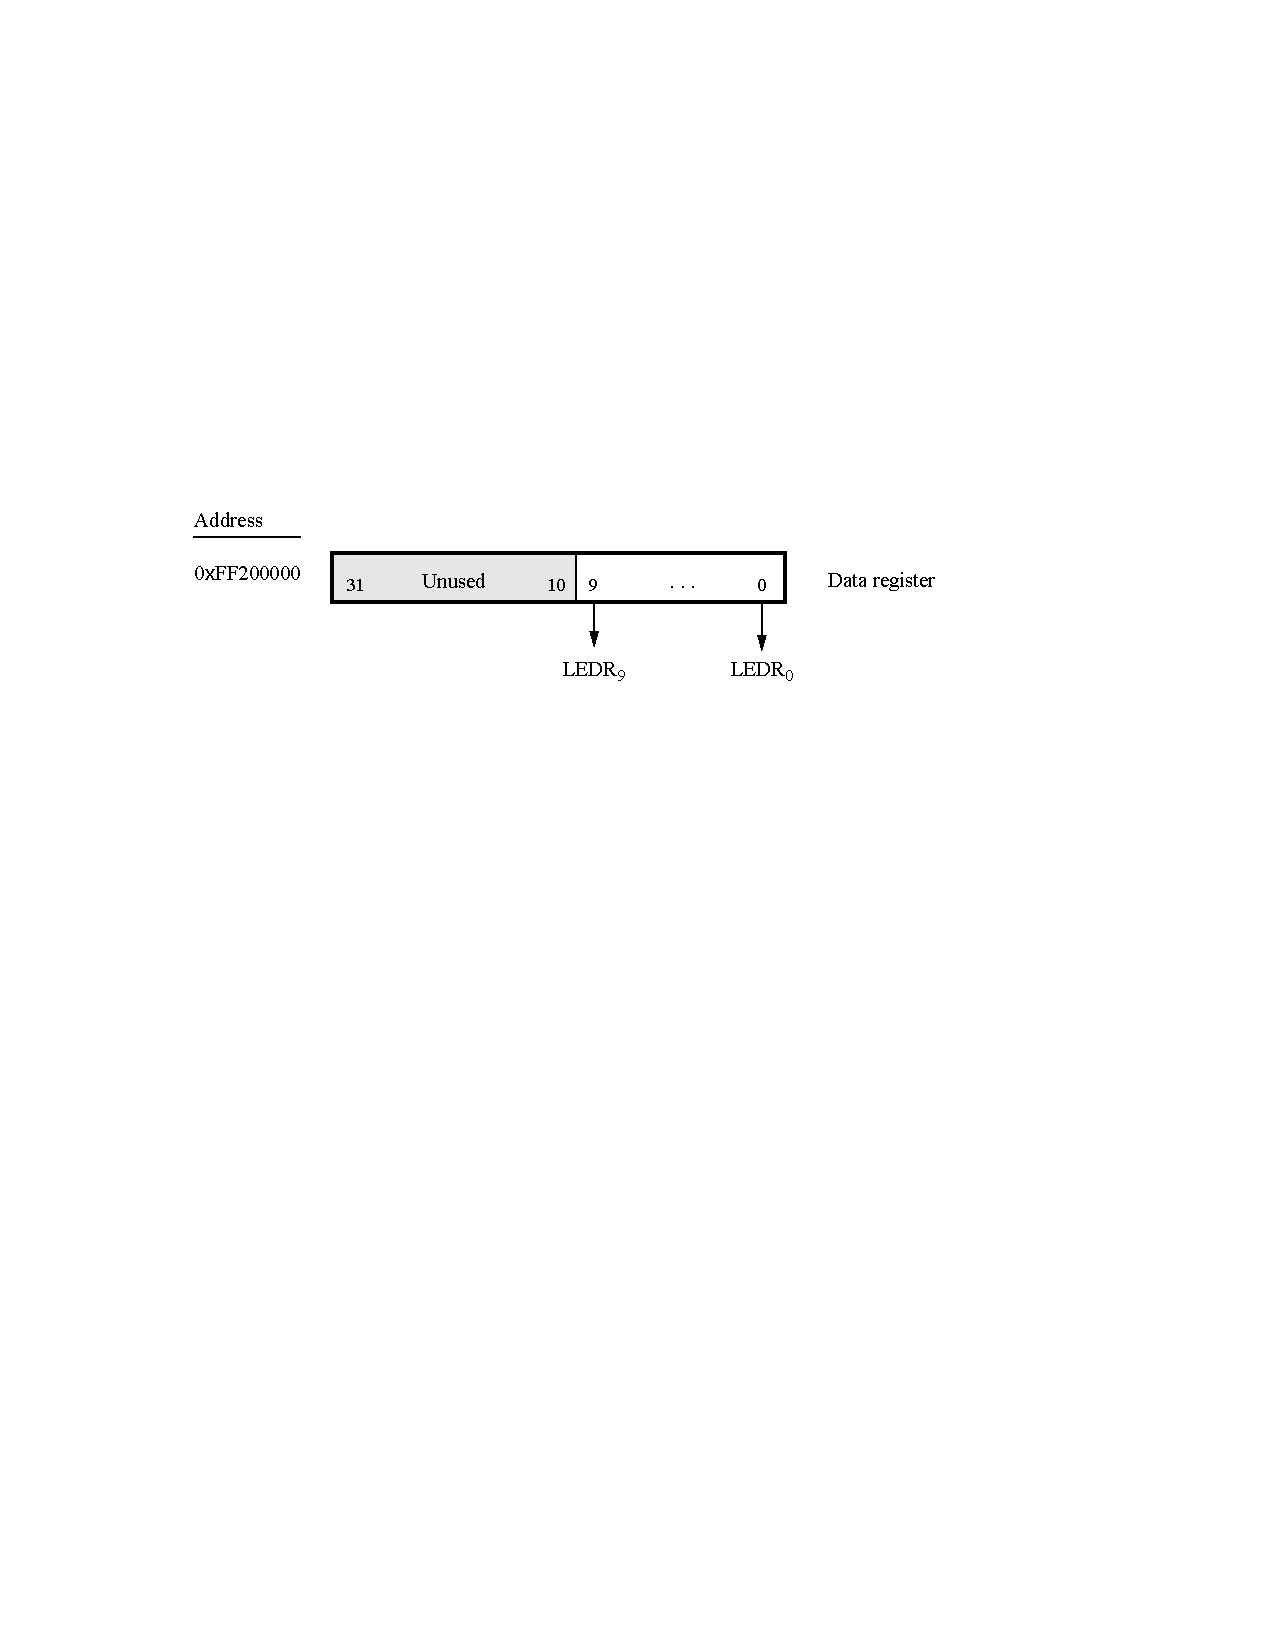
\includegraphics{figures/fig_LED_port.pdf}
   \end{center}
    \caption{The LEDR red light port.}
\label{fig:LEDR}

\end{figure}
\begin{figure}[H]
   \begin{center}
       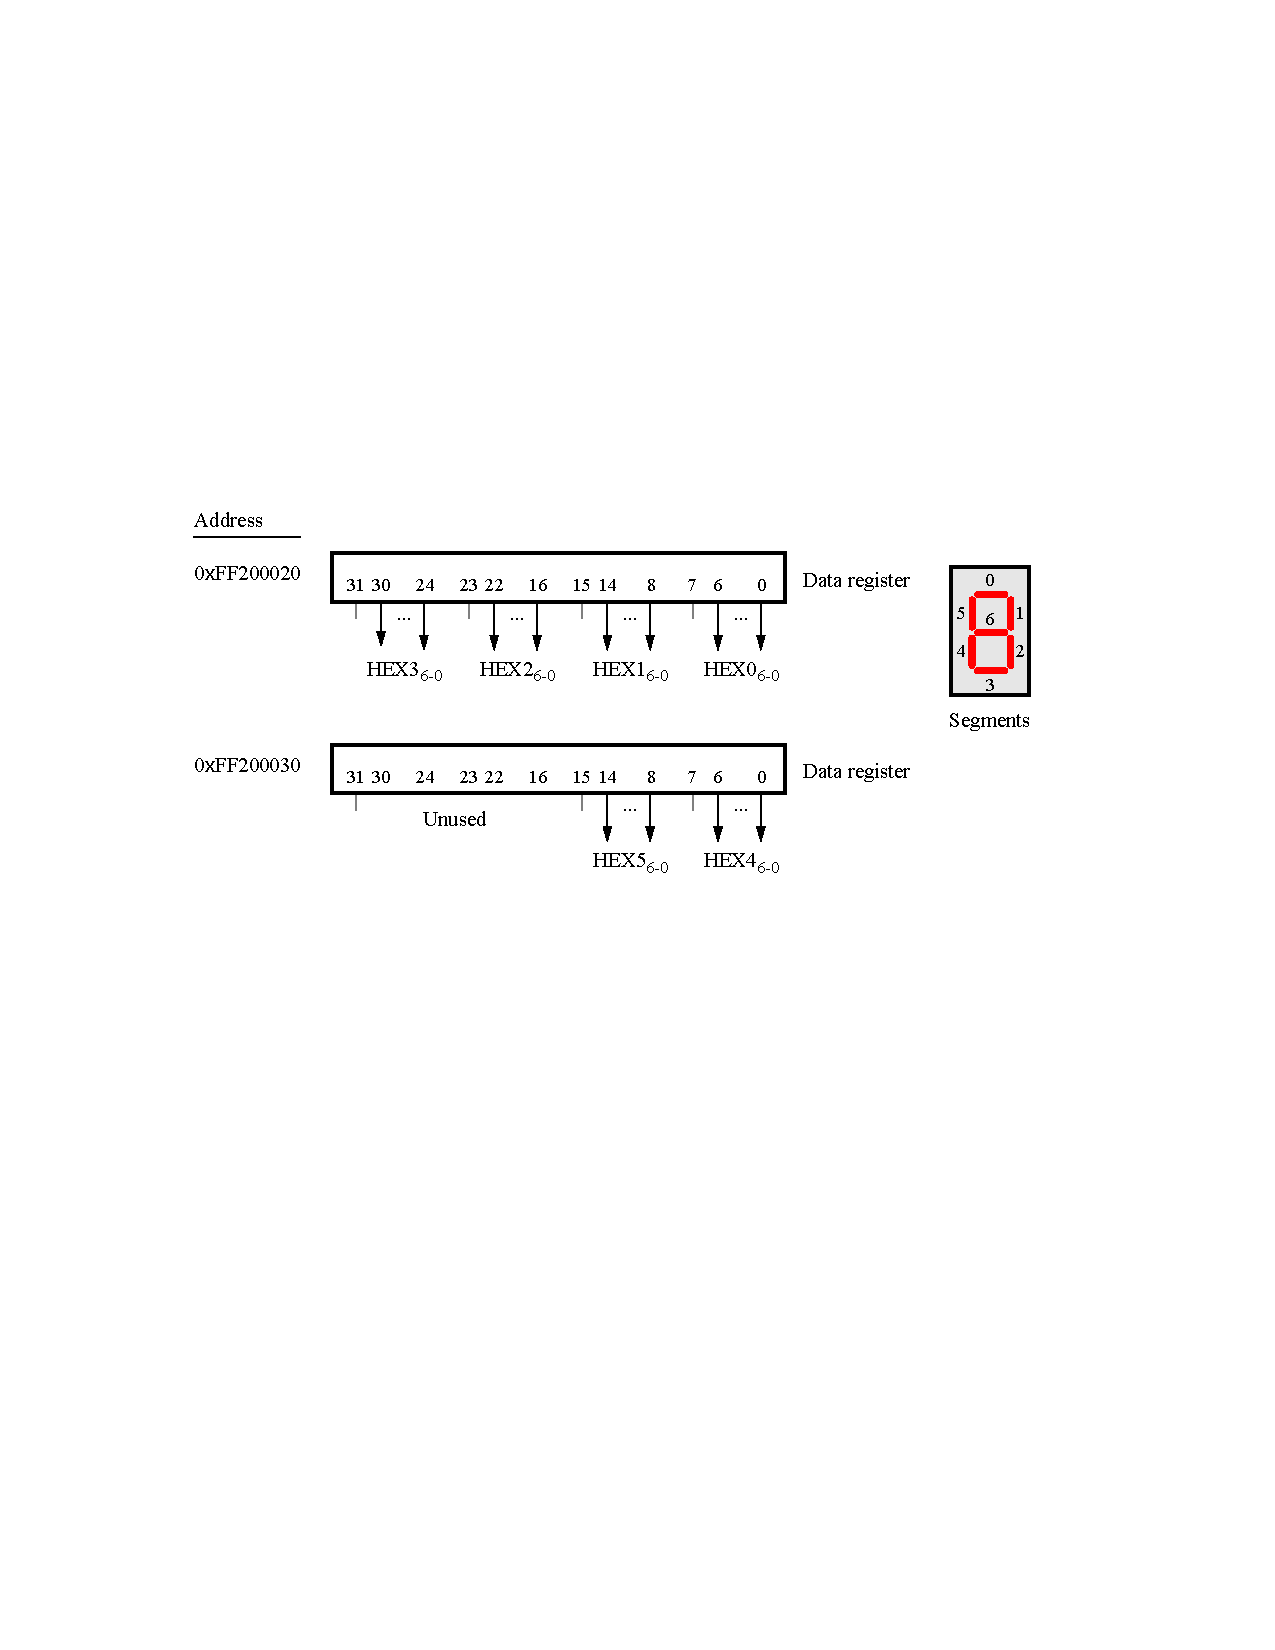
\includegraphics{figures/fig_segment_port.pdf}
   \end{center}
    \caption{The seven-segment display ports.}
\label{fig:HEX}
\end{figure}

\section*{Part IV}
\noindent
For this part you are to write a user-level program called {\it part4.c} that makes use of the 
character device drivers from Parts II and III. As we mentioned in Part III, if you are
using the DE10-Nano board, then ignore the parts of the solution that require
seven-segment displays. Perform the following:

\begin{enumerate}
\item In your program open the files /{\it dev}/{\it KEY} and /{\it dev}/{\it SW} for reading, 
and open the files /{\it dev}/{\it LEDR} and /{\it dev}/{\it HEX} for writing. Make a loop
in your program that does the following. Whenever a KEY is pressed capture the values of
the SW switches. Display these values on the LEDR lights. Also, keep a running
accumulation of the SW values that have been read, and show this sum on the HEX displays,
as a decimal value. 
\item Compile your program using a command such as \texttt{gcc -Wall -o part4 part4.c}.
\item Run your program and make sure that it works properly. Each time a KEY is
pressed, the values of the SW switches should immediately appear on the LEDR lights and the
sum should appear on the HEX displays. As an example, if the SW switches are set to 
$0000000101$, then the first time a KEY is pressed \red{000005} should be shown on the HEX 
displays, and the second time a KEY is pressed \red{000010} should be displayed.
\end{enumerate}
\vskip 0.8in
\newpage
%%%%%%%%%%%%%%%%%%%%%%%%%%%%%%%%%%%%%%%%
%%% FPGAcademy Copyright Information %%%
%%%%%%%%%%%%%%%%%%%%%%%%%%%%%%%%%%%%%%%%

%Always put the copyright on a new page (clear page), with some vertical space from top
\clearpage
\vspace{1in}

\noindent

Copyright {\copyright} FPGAcademy.org. All rights reserved. FPGAcademy and the 
FPGAcademy logo are trademarks of FPGAcademy.org.  This document is provided 
"as is", without warranty of any kind, express or implied, including but not 
limited to the warranties of merchantability, fitness for a particular purpose 
and noninfringement. In no event shall the authors or copyright holders be 
liable for any claim, damages or other liability, whether in an action of 
contract, tort or otherwise, arising from, out of or in connection with the 
document or the use or other dealings in the document.
~\\
~\\
**Other names and brands may be claimed as the property of others.



\end{document}
